\documentclass[tikz,border=12pt]{standalone}
\usepackage[T1]{fontenc}
\usepackage{mathpazo}
\usepackage{amsmath,amssymb}
\usetikzlibrary{arrows.meta, positioning, calc, fit, patterns, decorations.pathreplacing}

\definecolor{stblue}{HTML}{7B97AD}
\definecolor{rwgold}{HTML}{B8995E}
\definecolor{sage}{HTML}{7A9A7E}
\definecolor{dkbrown}{HTML}{3D3530}
\definecolor{wmgray}{HTML}{7B7067}
\definecolor{cream}{HTML}{F9F6F0}
\definecolor{border}{HTML}{D4C9B8}
\definecolor{terracotta}{HTML}{C47A6A}
\definecolor{lavender}{HTML}{907EA0}

\begin{document}
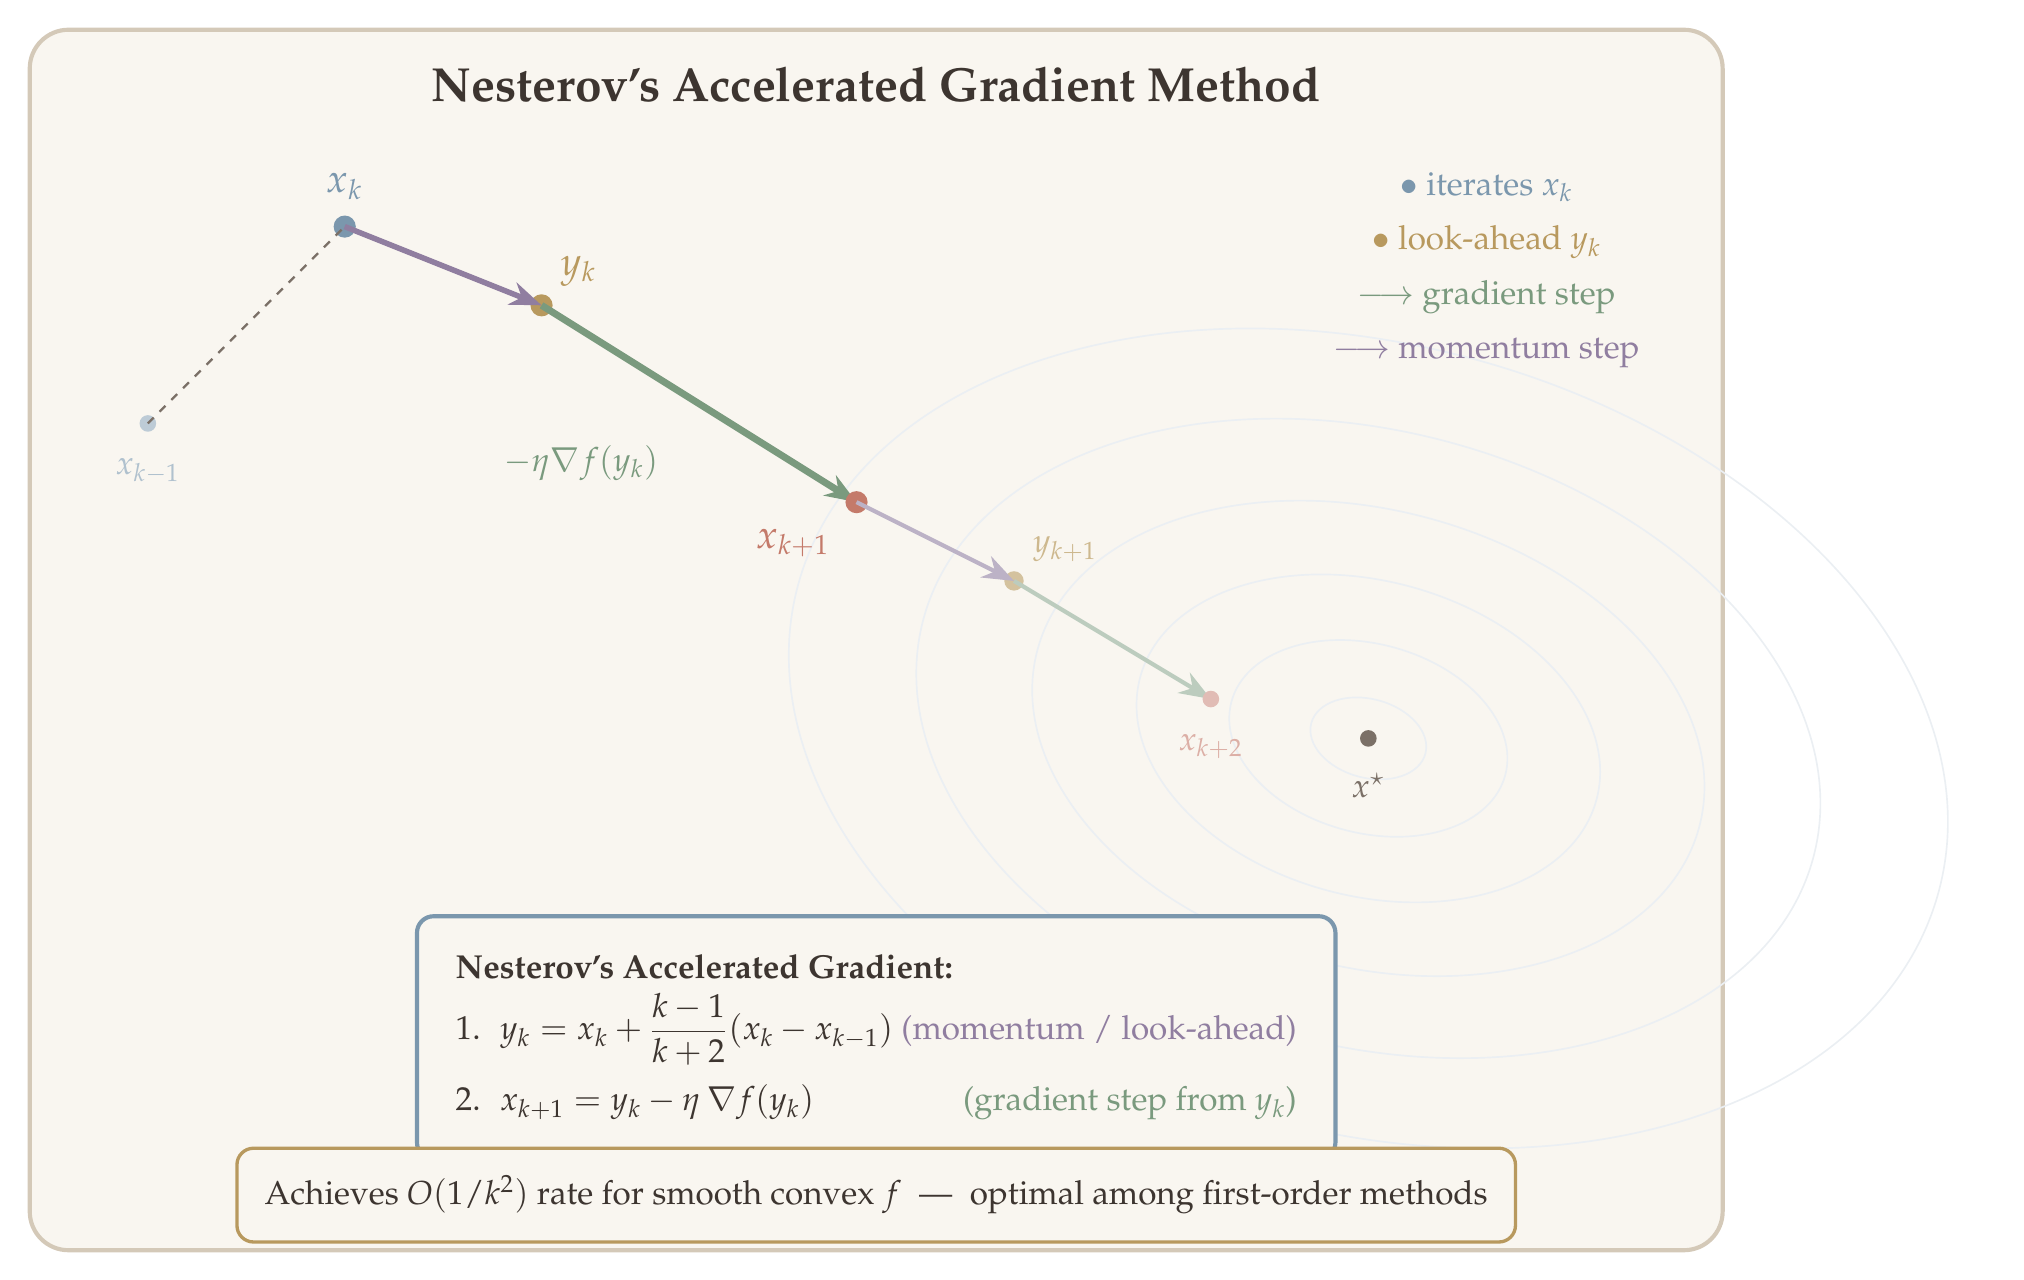
\begin{tikzpicture}[>={Stealth[length=4mm, width=3mm]}, line width=1.5pt]

% Background
\fill[cream, rounded corners=14pt] (-2,-4) rectangle (19.5,11.5);
\draw[border, line width=1.5pt, rounded corners=14pt] (-2,-4) rectangle (19.5,11.5);

% Title
\node[font=\LARGE\bfseries, text=dkbrown] at (8.75,10.8) {Nesterov's Accelerated Gradient Method};

% =========== Contour background ===========
\coordinate (opt) at (15,2.5);

\foreach \r in {0.5, 1.2, 2.0, 2.9, 3.9, 5.0} {
  \draw[stblue!15, line width=0.6pt, rotate around={-15:(opt)}]
    (opt) ellipse ({1.5*\r} and {\r});
}

% Optimum
\fill[wmgray] (opt) circle (3pt);
\node[font=\large, text=wmgray, below] at (15,2.2) {$x^\star$};

% =========== Legend (top right) ===========
\node[font=\large, text=stblue] at (16.5,9.5) {$\bullet$ iterates $x_k$};
\node[font=\large, text=rwgold] at (16.5,8.8) {$\bullet$ look-ahead $y_k$};
\node[font=\large, text=sage] at (16.5,8.1) {$\longrightarrow$ gradient step};
\node[font=\large, text=lavender] at (16.5,7.4) {$\longrightarrow$ momentum step};

% =========== Previous point x_{k-1} ===========
\coordinate (xkm1) at (-0.5,6.5);
\fill[stblue!50] (xkm1) circle (3pt);
\node[font=\large, text=stblue!60, below] at (-0.5,6.2) {$x_{k-1}$};

% =========== Iteration k ===========

% x_k
\coordinate (xk) at (2,9);
\fill[stblue] (xk) circle (4pt);
\node[font=\Large, text=stblue, above] at (2,9.2) {$x_k$};

% Dashed line from x_{k-1} to x_k
\draw[wmgray, dashed, line width=0.8pt] (xkm1) -- (xk);

% y_k (look-ahead)
\coordinate (yk) at (4.5,8.0);
\fill[rwgold] (yk) circle (4pt);
\node[font=\Large, text=rwgold, above right] at (4.6,8.1) {$y_k$};

% Momentum arrow: x_k -> y_k
\draw[->, lavender, line width=2pt] (xk) -- (yk);

% Gradient step: y_k -> x_{k+1}
\coordinate (xk1) at (8.5,5.5);
\draw[->, sage, line width=2.5pt] (yk) -- (xk1);

% Gradient label
\node[font=\large, text=sage, fill=cream, inner sep=3pt] at (5.0,6.0)
  {$-\eta\nabla f(y_k)$};

% x_{k+1}
\fill[terracotta] (xk1) circle (4pt);
\node[font=\Large, text=terracotta, below left] at (8.3,5.3) {$x_{k+1}$};

% =========== Iteration k+1 (faded) ===========

% y_{k+1}
\coordinate (yk1) at (10.5,4.5);
\fill[rwgold!60] (yk1) circle (3.5pt);
\node[font=\large, text=rwgold!70, above right] at (10.6,4.6) {$y_{k+1}$};

% Momentum from x_{k+1} to y_{k+1}
\draw[->, lavender!60, line width=1.5pt] (xk1) -- (yk1);

% Gradient from y_{k+1}
\coordinate (xk2) at (13,3.0);
\draw[->, sage!50, line width=1.5pt] (yk1) -- (xk2);

% x_{k+2}
\fill[terracotta!50] (xk2) circle (3pt);
\node[font=\large, text=terracotta!60, below] at (13,2.7) {$x_{k+2}$};

% =========== Algorithm box ===========
\node[fill=cream, draw=stblue, line width=1.5pt, rounded corners=6pt,
      font=\large, text=dkbrown, align=left, inner sep=14pt]
  at (8.75,-1.3) {%
  \textbf{Nesterov's Accelerated Gradient:}\\[4pt]
  1.\; $y_k = x_k + \dfrac{k-1}{k+2}(x_k - x_{k-1})$ \hfill {\color{lavender}(momentum / look-ahead)}\\[6pt]
  2.\; $x_{k+1} = y_k - \eta\,\nabla f(y_k)$ \hfill {\color{sage}(gradient step from $y_k$)}};

% Convergence note
\node[fill=cream, draw=rwgold, line width=1.2pt, rounded corners=6pt,
      font=\large, text=dkbrown, align=center, inner sep=10pt]
  at (8.75,-3.3) {Achieves $O(1/k^2)$ rate for smooth convex $f$ \;\textemdash\; optimal among first-order methods};

\end{tikzpicture}
\end{document}
